\chapter{Preliminaries}%{Philip Rideout}
\label{ch1}

%%%%%%%%%%%%%%%%%%%%%%%%%%%%%%%%
\section{WebGL and its Ancestry}
\summary{Gives an account of WebGL's ancestry (OpenGL, OpenGL ES), motivation, and rapid growth.  Also briefly mentions impediments at the time of writing, such as security concerns and IE support.}

3D graphics in the browser is not new.  One of the first technologies in this area was \index{VRML} VRML, the virtual reality modeling language standardized by the W3C in the mid 90's.  VRML was popular in academia but didn't quite have the same wildfire effect that characterizes the recent explosion of WebGL.

Why has WebGL left other 3D web technologies in the dust?  For one, it came along at just the right time; JavaScript only recently attained status as a serious platform for application development.  Sophisticated tools like Google's V8 \index{V8} engine  and John Resig's jQuery \index{jQuery} library have legitimized JavaScript in the eyes of developers coming from traditional desktop development.

WebGL has plenty of merits that make it more attractive than other browser-based 3D APIs.  Most desktop browsers support it natively, freeing users from the overhead of plug-ins.  WebGL is also ``close to the metal'' -- by providing low-level access to graphics hardware, developers can maximize performance like never before.

WebGL's ancestry actually lies not in VRML (which did give rise to X3D and other standards) but in a C-based graphics API created by Silicon Graphics in the early 90's.  They initially named their API \term{IrisGL}, which evolved to \term{OpenGL} when they released it as an industry standard.   With the rise of mobile platforms, OpenGL spawned \term{OpenGL~ES}, which encompasses almost the same feature set of WebGL.  In a sense, WebGL is simply a JavaScript binding for OpenGL ES 2.0.

Not long after Silicon Graphics released the first version of OpenGL to the world, a team of graphics scientists at Pixar were cooking up the \index{Renderman Shading Language}\term{Renderman Shading Language} to describe the materials used in their films.  RSL inspired much of the syntax in \term{GLSL}, the shading language added into OpenGL in the mid 2000's.  This is the same language that WebGL provides today for authoring shaders.  In the context of real-time graphics, \index{shaders}\term{shaders} are relatively small routines that get executed with massive parallelism.  Shaders have the final say in the 3D position of every vertex, and the RGB color of every rasterized pixel.  We'll learn more about shaders in Chapter~2.

%%%%%%%%%%%%%%%%%%%%%%%%%%%%%%%%%%%%%%%%%%%%%

\section{Requirements}

In terms of development tools, WebGL has a low barrier to entry. You don't need to download a fancy IDE or grapple with installation of libraries and plug-ins.  It doesn't matter if you use a Mac, Windows, or Linux.  And, since WebGL is a subset of a native graphics API, you don't necessarily need a high-powered GPU either.  All you need is a text editor and a modern web browser!

At the time of this writing, the latest versions of Firefox, Chrome, and Safari all support WebGL natively in their desktop variants.  We've tested Giza on all three of these browsers, but we found Chrome to have the best performance and extension support.

Support for mobile platforms such as iOS and Android isn't quite here  yet, but that may change by the time you read this.

With Safari, you may need to explicitly enable WebGL.  Go to \textbf{Safari~>~Preferences}.  In the Advanced tab, make sure the develop menu is enabled.  Now you should be able to select \textbf{Develop~>~Enable~WebGL}.

For those interested in supporting Internet Explorer, there's a plugin you can try:

\url{http://iewebgl.com/}

No matter which browser you choose, your best friend will quickly become its \term{Development Console}.  Find it and get acquainted if you're not already.  It's the place for setting breakpoints, examining the call stack, and viewing diagnostic output.  In our sample code, we tend to print diagnostic messages using JavaScript's \code{console} object rather than calling the \code{alert} function; these messages are only visible in the development console.

%%%%%%%%%%%%%%%%%%%%%%%%%%%%%%%%%%%%%%%%%%%%%

\section{Building Giza}
\summary{Describes our coding conventions and the \code{giza} library that is developed over the course of the book.}

\begin{figure}[htb]\centering
  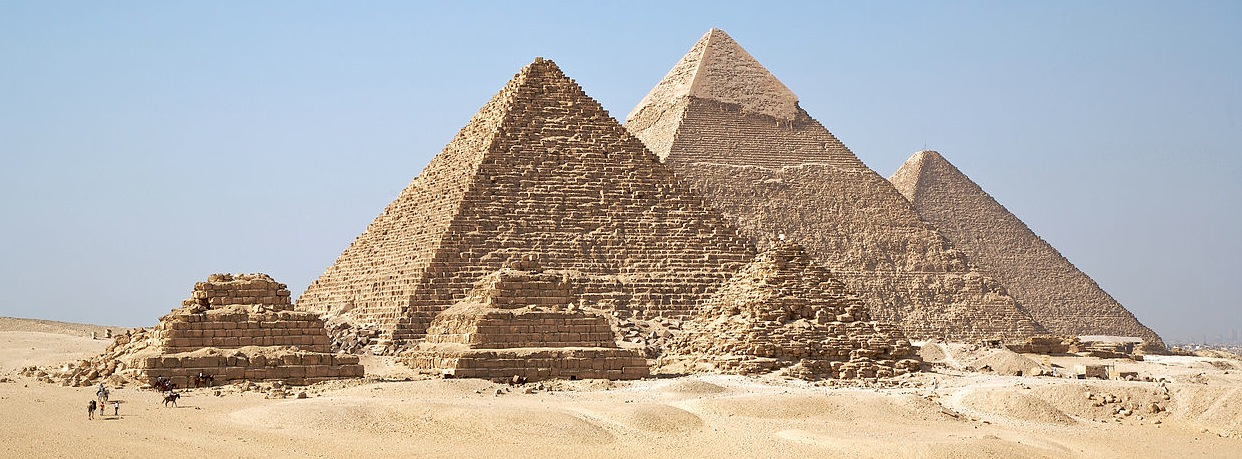
\includegraphics[width=70mm]{All_Gizah_Pyramids.jpg}
  \caption{The silhouette of the Giza pyramids is composed of triangles, the fundamental drawing primitive in real-time graphics. (Ricardo Liberato)}
  \label{fig:Giza}
\end{figure}

This is not just a book, it's a library.  Many of the code listings on these pages are lifted directly from the giza library, named after the ancient Egyptian city.  The Giza pyramids form a skyline of triangles, which are the primary drawing primitive in WebGL.  The pyramid shape also describes a \term{viewing frustum}, a spatial region that encompasses everything within a certain vantage point in a 3D graphics program.

As a design philosphy, giza rarely calls methods on the WebGL context object -- that's your job!  This differentiates it from higher-level libraries such as ThreeJS.  Instead of providing an abstraction of WebGL, giza offers a set of utility layers that help with vector algebra, building mesh data, and implementing 3D manipulator widgets.

\subsection{Code Conventions}

All giza methods belong to a global object called \code{GIZA}, following the namespace convention common in JavaScript.  For example, here's how we define a small utility function that merges all attributes from object \code{b} into object \code{a}:

\begin{lstlisting}[language=JavaScript]
var GIZA = GIZA || {};

GIZA.merge = function (a, b) {
  for (var attrname in b) {
    a[attrname] = b[attrname];
  }
  return a;
};
\end{lstlisting}

The first line is repeated at the top of all giza files.  This allows clients to include a subset of giza because it creates a new \code{GIZA} namespace only if it doesn't already exist.

Other than \code{GIZA}, the only global variable that we create is \code{COMMON}.  This is where we place a small handful of WebGL helpers.  Unlike methods in \code{GIZA} -- which have no dependencies on third-party libraries) -- methods in \code{COMMON} are allowed to call jQuery functions and WebGL methods.

To reduce code verbosity, we'll often create short-named aliases at the top of a scope.  For example:

\begin{lstlisting}[language=JavaScript]
var V3 = GIZA.Vector3;
var gl = GIZA.context;
...
gl.clear(gl.COLOR_BUFFER_BIT);
var p = V3.subtract(a, V3.normalized(b));
\end{lstlisting}

Note that we capitalize namespace objects, and we use lowercase for instanced variables.  You'll agree that the above code is preferable to:

\begin{lstlisting}[language=JavaScript]
GIZA.context.clear(GIZA.context.COLOR_BUFFER_BIT);
var p = GIZA.Vector3.subtract(a, GIZA.Vector3.normalized(b));
\end{lstlisting}

For access to the full source code to giza, or to download the minified library, refer to our github site:

\notetoself{\url{http://to.be.filled.in.com}}

The github project also contains code for all the samples in this book, including HTML and CSS source (and the \code{COMMON} layer).

%%%%%%%%%%%%%%%%%%%%%%%%%%%%
\section{The Canvas Element}
\summary{Explains the \code{width} and \code{height} attributes and how to handle high-dpi displays (e.g., Apple Retina).}

The canvas element \index{\code{<canvas>} element} is one of the cornerstones of the HTML5 platform.  It provides rich drawing APIs for both 2D and 3D graphics.  The 2D API will not be discussed much in this book (except briefly in \notetoself{CHAPTER}), and the 3D API is, of course, WebGL.

\subsection{Dealing with Size}

By default, \code{<canvas>} is a block level element, similar to \code{<div>}.  This means that it can only be a child of \code{<body>}, and that it's typically rendered with surrounding line breaks.

An important distinction between canvas and other elements is that it has two \index{size} sizes.  One size is the \term{display area}, specified with familiar \index{CSS} CSS mechanisms.  The other size is the \term{content size}, specified with explicit \code{width} \index{\code{width} attribute} and \code{height} \index{\code{height} attribute} attributes.  The content size specifies an off-screen drawing surface that gets scaled into the display area on the web page.

It's tempting to simply set the content and display sizes to the same dimensions, as in:

\begin{lstlisting}[language=HTML]
<canvas style="width:640px; height:360px"
        width="640" height="360">
</canvas>
\end{lstlisting}

There's nothing wrong with the above approach for simple applications.  It's common, however, to specify a dynamic display area (e.g., \code{width:100\%}).  Moreover CSS pixels don't necessarily correspond to actual device pixels.  This is especially true on displays with a high pixel density, where browsers typically upscale CSS pixels by 2x.

\begin{sidenote}%
Watch out!  If you assume that device pixels are 1:1 with CSS pixels, some users might see bluriness in the WebGL canvas due to upscaling.
\end{sidenote}

To get around these issues, \code{GIZA.init} (Listing~\ref{lst:GIZA:init1}) examines the \linebreak \code{devicePixelRatio} window property to check how much upscaling is active.  It also examines the \code{clientWidth} \index{\code{clientWidth}, \code{clientHeight}} and \code{clientHeight} properties of the canvas element to obtain the finalized display area.

\begin{lstlisting}[
    caption={Adjusting the canvas size.},
    label=lst:GIZA:init1,
    language=JavaScript]
GIZA.init = function(canvasElement) {

  // Find a canvas element if one wasn't specified.
  var canvas = canvasElement;
  if (!canvas) {
    canvas = document.getElementsByTagName('canvas')[0];
  }

  // Obtain the browser's upscale amount, assuming 1 if unavailable.
  var pixelScale = window.devicePixelRatio || 1;

  // Define a function that adjusts content size.
  var adjustSize = function() {
    var displayWidth = canvas.clientWidth;
    var displayHeight = canvas.clientHeight;
    canvas.width = displayWidth * pixelScale;
    canvas.height = displayHeight * pixelScale;
  };

  adjustSize();
  window.onresize = adjustSize;
\end{lstlisting} \index{\code{GIZA.init}}

In Listing~\ref{lst:GIZA:init1}, we adjust the canvas width and height not only during initialization, but also in response to the window's \index{\code{onresize} event} \code{onresize} event.  (It's also common to adjust the WebGL \term{viewport} and \term{projection matrix} during a resize event, but we'll learn more about that in future chapters.)

By using the above initialization strategy, the HTML side of your app can skip setting the explicit \code{width} and \code{height} attributes, opting instead for a purely CSS-based approach:

\begin{lstlisting}[language=HTML]
<canvas style="width:100%; height:360px">
</canvas>
\end{lstlisting}

\subsection{Getting a Context}
\label{sec:context}

The entire WebGL API is exposed through a \code{WebGLRenderingContext} \index{\code{WebGLRenderingContext}} object, commonly known as the \index{draw context} \term{draw context}.  It's obtained by calling \code{getContext} \index{\code{getContext} method} on a canvas element, like so:

\begin{lstlisting}[language=JavaScript]
  gl = canvas.getContext('experimental-webgl', {antialias: true});
\end{lstlisting}

At the time of this writing, \code{"experimental-webgl"} \index{\code{experimental-webgl}} is the only string that can be passed to \code{getContext} for WebGL.  (For the 2D canvas API, the string \code{"2d"} is used.)

The second argument is a set of optional attributes, as specified in Table~\ref{tab:ContextAttributes}.

\begin{table}[htb]\centering
  \begin{tabular}{lll}
    \hline
    Key & Default & Description \\
    \hline
    alpha & true & Alpha channel \\
    depth & true & Depth buffer \\
    stencil & false & Stencil buffer \\
    antialias & true & Enables multisampling \\
    premultipliedAlpha & true & Specifies compositing behavior \\
    preserveDrawingBuffer & false & Retains canvas image previous draw cycle \\
    \hline
  \end{tabular}
  \caption{WebGL context options.}
  \label{tab:ContextAttributes}
\end{table}

We'll examine these attributes in greater detail in the next section.

\notetoself{Add references to future sections in the book that deal with context loss and image capture.}

\subsection{Clearing the Canvas}

The only WebGL functions discussed in this chapter are the first two methods listed in Table~\ref{tab:Clearing}.

\begin{table}[htb]\centering
  \begin{tabular}{ll}
    \hline
    Method & Argument Types \\
    \hline
    clear(mask) & logical ``or'' of values from Table~\ref{tab:ClearBit} \\
    clearColor(red, green, blue, alpha)  & floating point numbers in [0,1] \\
    clearDepth(value) & floating point number in [0,1] \\
    clearStencil(mask) & integer \\
    \hline
  \end{tabular}
  \caption{WebGL clear methods.}
  \label{tab:Clearing}\index{\code{clear}}\index{\code{clearColor}}\index{\code{clearDepth}}\index{\code{clearStencil}}
\end{table}

The \code{clear} method resets all the pixels in the canvas.  The \code{clearColor}, \code{clearDepth}, and \code{clearStencil} methods are used to configure subsequent calls to \code{clear}.  In other words, they are \term{state-setting methods}.  Most of the WebGL API consists of state-setting methods; in fact there are only three methods in the entire API that actually paint pixels rather than setting state:

\begin{description}
\item[\code{clear}] Fills the color buffer (or depth/stencil).
\item[\code{drawArrays}] Draws 3D geometry defined by a sequential list of vertices.
\item[\code{drawElements}] Draws 3D geometry defined by a list of indices into a vertex buffer.
\end{description}

We'll learn more about \code{drawArrays} and \code{drawElements} in the next chapter.  Listing~\ref{lst:ClearCanvas} shows a usage example for the \code{clear} method.  It fills the canvas with solid yellow.

\begin{lstlisting}[
    caption={Clearing the canvas.},
    label=lst:ClearCanvas,
    language=JavaScript]
gl = canvas.getContext('experimental-webgl', {antialias: true});
gl.clearColor(1, 1, 0, 1);
gl.clear(gl.COLOR_BUFFER_BIT);
\end{lstlisting}

The \code{COLOR\_BUFFER\_BIT} flag is one of the constants that can be combined with a logical ``or'' to specify which drawing layers to include in the canvas.  To reduce the memory footprint, choose the fewest number of flags from Table~\ref{tab:ClearBit}.  In fact, don't worry about the depth and stencil layers just yet; we'll learn more about them in future chapters.

\begin{table}[htb]\centering
  \begin{tabular}{lll}
    \hline
    Property & Value & Default Value \\
    \hline
    \code{DEPTH\_BUFFER\_BIT}   & 0x0100 & 0.0 \\
    \code{STENCIL\_BUFFER\_BIT} & 0x0400 & 0x00000000\\
    \code{COLOR\_BUFFER\_BIT}   & 0x4000 & (0, 0, 0, 0) \\
    \hline
  \end{tabular}
  \caption{WebGL clear bits.}
  \label{tab:ClearBit}
\end{table}

You can find a \code{clear} call in most of the code samples in this book, but keep in mind that it's not always required.  Some applications never bother filling the background with a solid color.

For example, consider a game inside an infinite tunnel, as depicted on the far left in Figure~\ref{fig:Tunnel}.  Since every pixel in the canvas is affected by 3D drawing commands, there's no need to clear the color buffer.  If, however, the tunnel were finite (middle panel), there would be an area of the screen that never gets updated.  If you don't explicitly clear the canvas before drawing, the unpainted region might contain a ``dirty'' image (right panel), depending on the \code{preserveDrawingBuffer} option you chose when creating the context.  More on this in the next section.

\begin{figure}[htb]\centering
  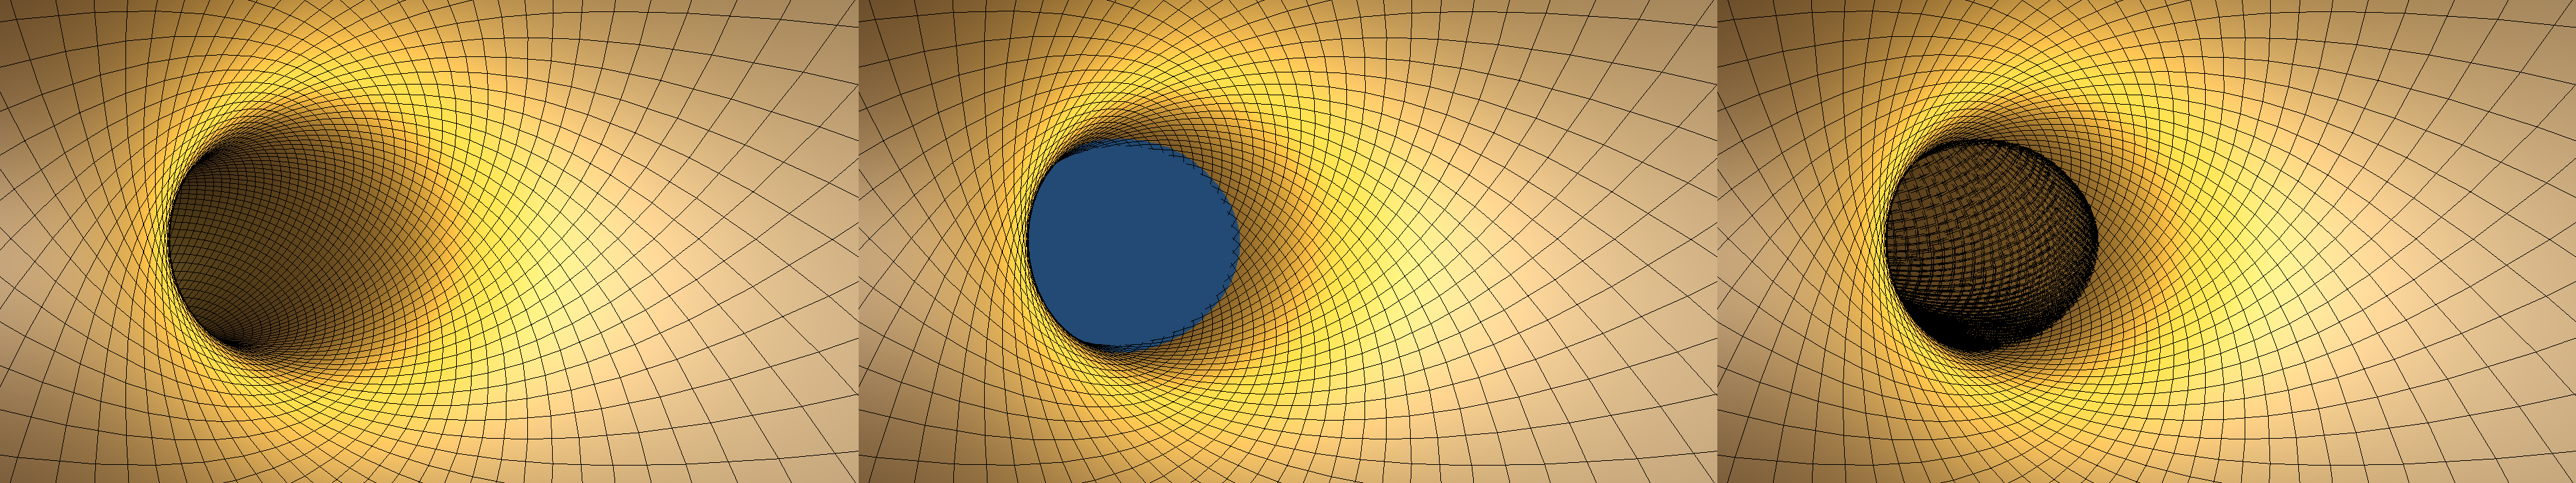
\includegraphics[width=120mm]{Tunnels.png}
  \caption{The effects of \code{clear()} and \code{preserveDrawingBuffer}.  The closed tunnel on the far left does not need \code{clear()}.}
  \label{fig:Tunnel}
\end{figure}\index{tunnel}

\subsection{When is the canvas \emph{truly} updated?}
\label{sec:doublebuffer}

You might be familiar with \index{double-buffering} double-buffering if you've used other graphics APIs.  WebGL is always double-buffered.  This means that your drawing commands are actually affecting pixels in a \index{backbuffer} \term{backbuffer}, which is an offscreen drawing surface.  The browser's render loop presents the finalized backbuffer to the screen in one fell swoop.  This creates the illusion of seamless animation by never allowing users to see a partially complete scene.

One side effect of double-buffering is that that the existing pixels you're overwriting do not necessarily correspond to what was drawn in the previous frame.  Normally this doesn't matter; most applications either clear the existing buffer, or fill it entirely with 3D drawing primitives.

In some situations you want the existing pixels to exactly match the previously-drawn frame.  For example, you might need to read color values from the canvas (the \index{\code{readPixels}} \code{readPixels} method will be discussed in \notetoself{CHAPTER}), or your application might intentionally update only certain regions of the canvas for performance reasons.  This is why \code{preserveDrawingBuffer} exists; it allows you to mimic \index{single-buffering} single-buffering.

You might be thinking: ``Okay, so the canvas isn't immediately updated when I call \code{clear} or \code{drawPixels}, but the \emph{backbuffer} is!''  Nope -- the web browser and the graphics driver are actually buffering up WebGL commands and executing them later.  If you'd like, you can tell WebGL to wait till the buffer is done executing by calling the \index{\code{finish}} \code{finish} method.  You'll rarely need this however, so don't use it unless you know you need it.

\subsection{Alpha Compositing}

If you're reading this book, you probably already know about the alpha channel, invented in the late 70's by Alvy Ray Smith, one of the co-founders of Pixar Animation Studios.

Alpha is usually a floating-point value in the [0,1] interval, treated much like the red, green, and blue components of pixel color.  Alpha can be thought of as the inverse of opacity, although WebGL can interpret it in many ways, as we'll learn in \notetoself{CHAPTER}.  For now we'll focus on how the alpha channel in the canvas interacts with the page compositor in your browser.

Consider the case where the canvas is cleared to a half-opaque red color like so:

\begin{lstlisting}[language=JavaScript]
gl.clearColor(1, 0, 0, 0.5);
gl.clear(gl.COLOR_BUFFER_BIT);
\end{lstlisting}

If the \code{premultipliedAlpha} option is disabled upon context creation, the RGB values in the canvas are multiplied by alpha before being added into the underlying color, as seen on the right in Figure~\ref{fig:PreMult}.

Another example would be clearing the background to (1, 1, 1, 0.5).  If \code{premultipliedAlpha} were enabled in this case, the canvas would be completely opaque because adding white to any color yields white.  If \code{premultipliedAlpha} were disabled, this would (crudely) brighten the background by averaging it with white.

\begin{figure}[htb]\centering
  \includegraphics[width=120mm]{PreMult.png}
  \caption{Semi-transparent canvas composed over a CSS \code{background-image}.}
  % http://en.wikipedia.org/wiki/File:BYR_color_wheel.svg
  \label{fig:PreMult}
\end{figure}

If the \code{alpha} option is disabled when creating a context, none of this matters -- the \code{premultipliedAlpha} option is ignored.  The \code{alpha} option is enabled by default, as is \code{premultipliedAlpha}.

\begin{comment}
Note that we're not addressing css-opacity.

In this book, we never add children elements to \code{<canvas>}, but there's nothing wrong with doing so.  On some platforms, this can degrade performance, although this is improving as WebGL implementations are maturing.

http://www.svgopen.org/2005/papers/abstractsvgopen/
http://stackoverflow.com/questions/9491417/when-webgl-decide-to-update-the-display?answertab=votes#tab-top

\end{comment}

%%%%%%%%%%%%%%%%%%%%%%%%%%
\section{Animation Timing}
\summary{How to periodically trigger draw events.}

You wouldn't be learning WebGL unless you were interested in animation.  WebGL applications generally issue all rendering commands for a given 3D scene in a \term{draw cycle}.  The easiest but most naive way of doing this in JavaScript is \code{setInterval}:

\begin{lstlisting}[language=JavaScript]
// Call myDrawFunc() every 60th of a second
var delay = 1 / 60;
window.setInterval(myDrawFunc, delay / 1000);
\end{lstlisting}

The above approach is hardly ideal for high-performing 3D graphics.  It's preferable to hook in to the browser's native rendering loop.  This allows your animation routine to become idle if the browser has no need to draw itself (e.g., if the window is minimized), saving precious battery life and CPU cycles.  It also aligns your animation with the refresh rate of the monitor, preventing chopiness.

At the time of this writing, all major browsers supply a method on \code{window} exactly for this purpose, although it has a vendor-specific prefix until it becomes fully standardized.  Giza's \code{init} function handles this for you, as seen in Listing~\ref{lst:GIZA:init2}.

\begin{lstlisting}[
    caption={Initializing \code{requestAnimationFrame}.},
    label=lst:GIZA:init2,
    escapechar=\%,
    language=JavaScript]
GIZA.init = function(canvasElement) {

  ...

  window.requestAnimationFrame = window.requestAnimationFrame ||
    window.mozRequestAnimationFrame ||
    window.webkitRequestAnimationFrame ||
    window.msRequestAnimationFrame;
\end{lstlisting} \index{\code{GIZA.init}}

The \code{requestAnimationFrame} method is actually more like \code{setTimeout} than \code{setInterval} because it doesn't automatically repeat itself.  Typically this means you'll want to call it during your draw cycle.  Giza wraps this functionality by providing the \code{endFrame} function, meant to be called at the end of your draw function. See Listing~\ref{lst:GIZA:endFrame}.

\begin{lstlisting}[
    caption={Common end-of-frame tasks.},
    label=lst:GIZA:endFrame,
    language=JavaScript]
GIZA.endFrame = function(drawFunc) {
  var err = gl.getError();
  if (err != gl.NO_ERROR) {
    console.error("WebGL error during draw cycle: ", err);
    // Don't request another draw cycle here;
    // this prevents an infinite cascade of errors.
  } else {
    window.requestAnimationFrame(drawFunc, GIZA.canvas);
  }
};
\end{lstlisting} \index{\code{GIZA.endframe}}

In addition to requesting the next animation cycle, it also checks the WebGL error state and halts animation if an error occurs.  This is good practice to maintain clean, error-free code.

See Listing~\ref{lst:drawFunc} for a usage example.  All recipes will have this basic structure.

\begin{lstlisting}[
    caption={High-level structure of a Giza application.},
    label=lst:drawFunc,
    language=JavaScript]
var draw = function(time) {
  // do work here...
  GIZA.endFrame(draw);
}

GIZA.init();
draw(GIZA.getTime());
\end{lstlisting}

Note that we explicitly called \code{draw} function after initialization to kick off the animation cycle.  Giza provides a \code{getTime} method to provide a timestamp that's consistent with the time argument provided to \code{requestAnimationFrame}.

%%%%%%%%%%%%%%%%%%%%%%%%%%%%%%%%
\rrecipe{Recipe 1: Strobe Light}
\summary{The simplest possible WebGL application; animates a solid color with \code{clear}.}

Every chapter in this book ends with a \term{recipe} that walks through all the code for a certain giza demo.  Each recipe has a very simple page layout, as seen in Figure~\ref{fig:Recipe1}.

\begin{figure}[htb]\centering
  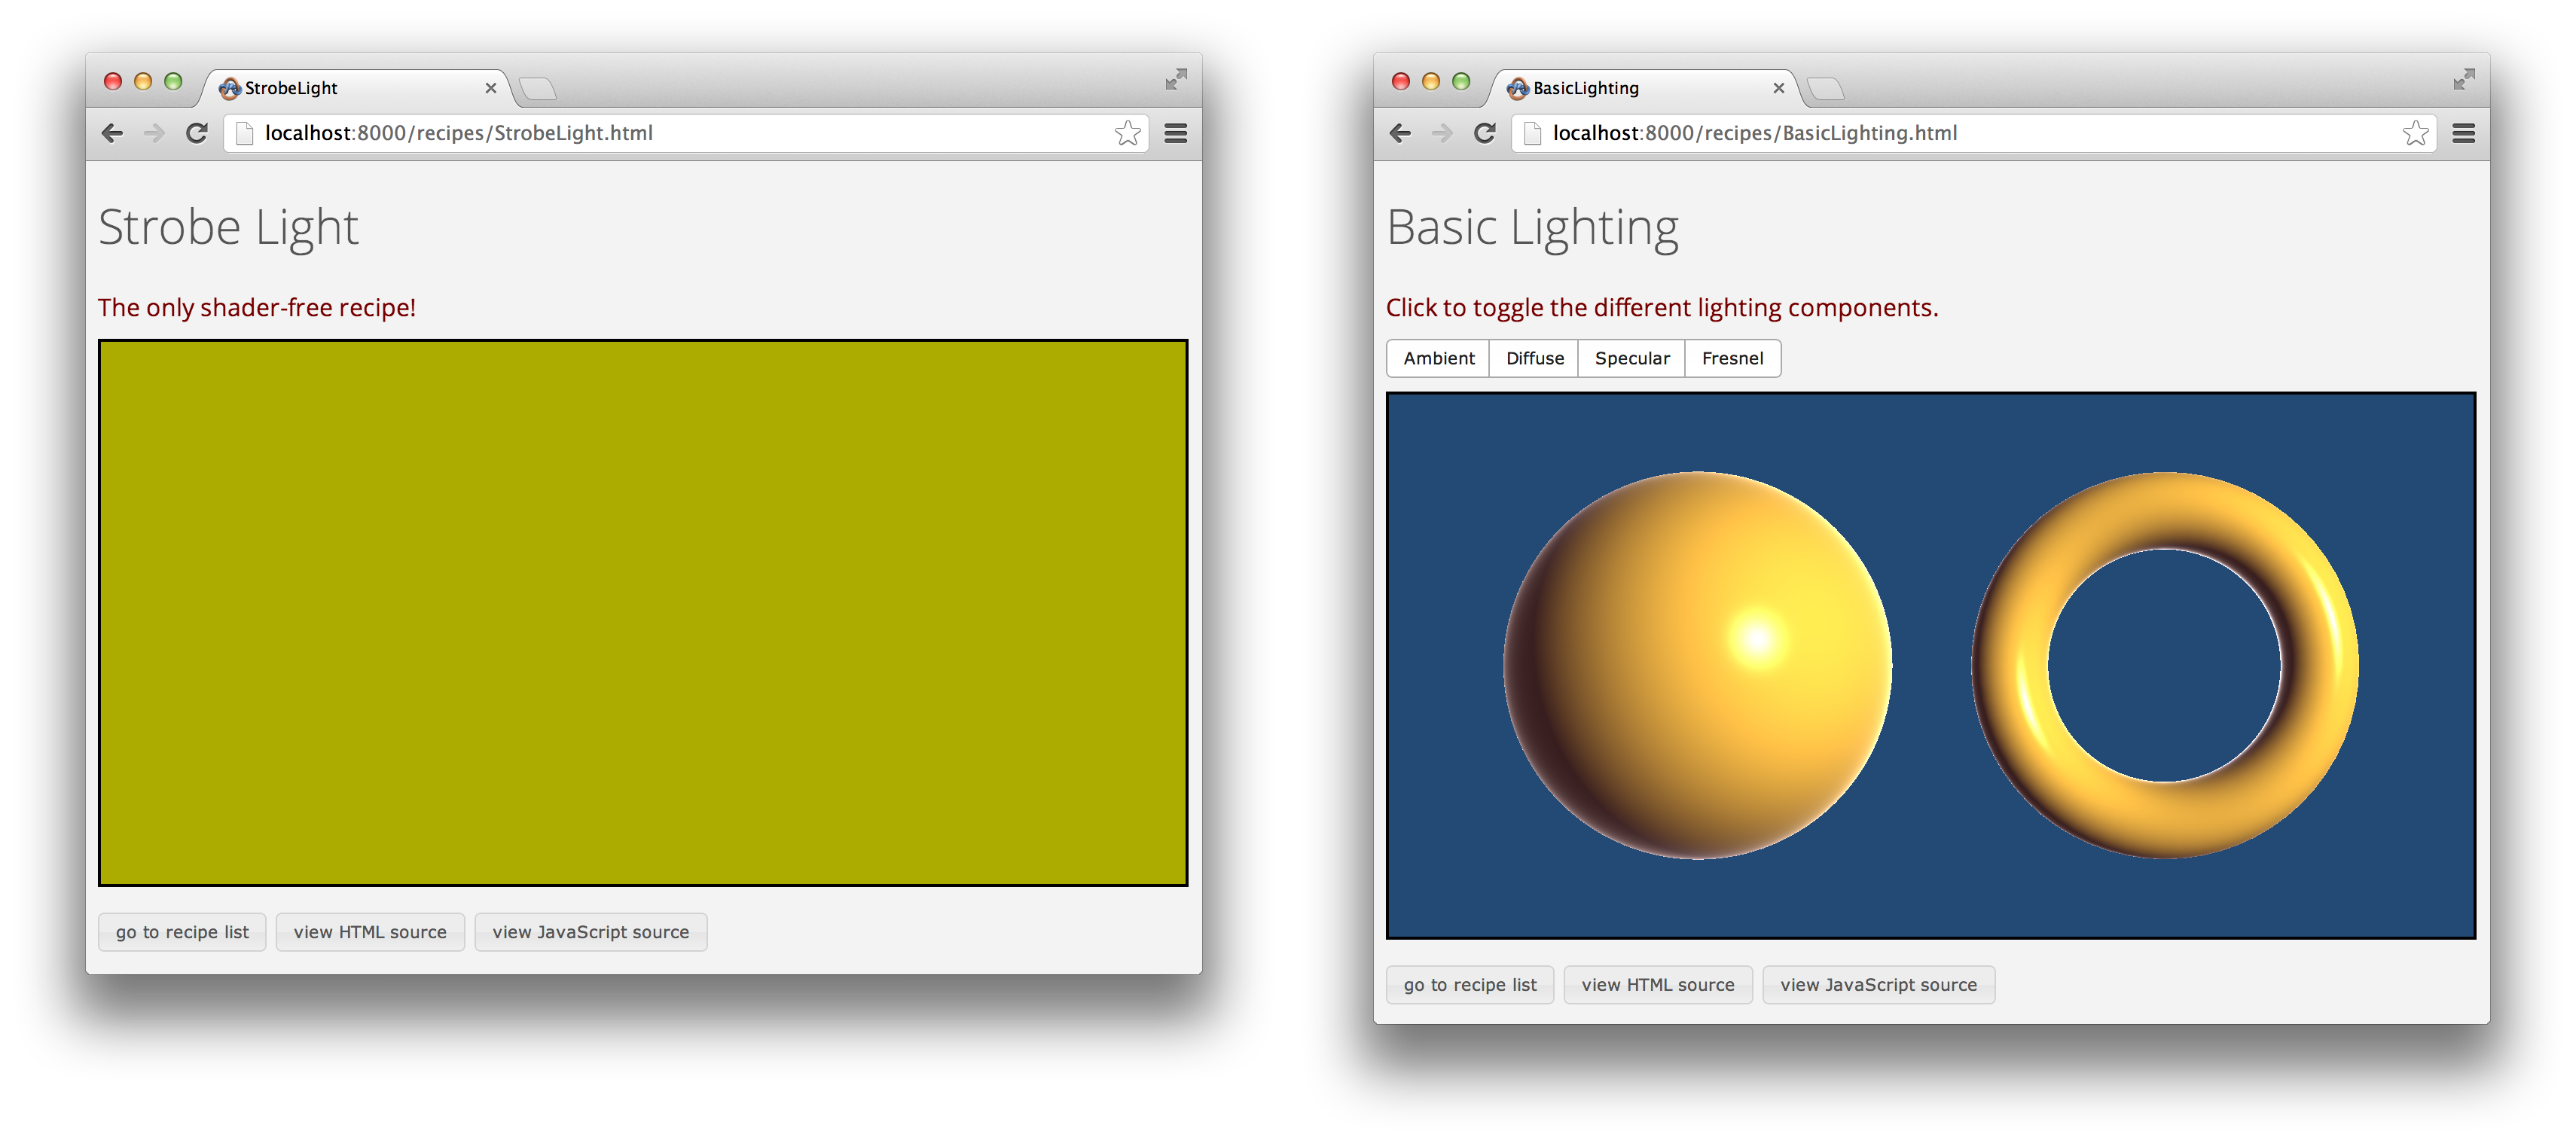
\includegraphics[width=120mm]{Recipe1.png}
  \caption{Examples of recipes: \code{StrobeLight} from Chapter 1 and \code{BasicLighting} from Chapter 4.}
  \label{fig:Recipe1}
\end{figure}

This chapter's recipe is called \code{StrobeLight}, which isn't very exciting but at least establishes some boilerplate for future recipes.  Take a look at the HTML in Listing~\ref{lst:StrobeLight1}.

\begin{lstlisting}[
    caption={\code{StrobeLight.html}},
    label=lst:StrobeLight1,
    language=HTML]
<!DOCTYPE html>
<html lang="en">
  <head>
    <title>StrobeLight</title>
    <link href="css/style.css" rel="stylesheet">
    <script src="lib/head.load.min.js"></script>
    <script src="common.js"></script>
  </head>
  <body>
    <h1>Strobe Light</h1>
    <div class="tagline">
      The only shader-free recipe!
    </div>
    <canvas style="width:640;height:360px">
    </canvas>
    <div id="button-bar">
    </div>
  </body>
</html>
\end{lstlisting} \index{\code{StrobeLight.html}}

While giza has no dependencies on any JavaScript libraries, the \code{COMMON} layer depends on the following third-party libraries to make life a little easier:

\begin{description}
\item[head.js] Resource loading library from Tero Piirainen.  We use a minified subset called \texttt{head.load.min.js}.
%\item[stats.js] Performance monitoring widget used in some recipes, written by Ricardo Cabello of ThreeJS fame.
\item[jQuery] John Resig's insanely popular ``write less do more'' library.
\end{description}

HeadJS enables us to simplify the HTML by sharing a list of JavaScript libraries in \code{common.js} instead of duplicating a large set of \code{<script>} tags in every HTML file.  It also has the benefit of loading scripts asynchronously for better performance.  See Listing~\ref{lst:COMMON:file} for \code{common.js}.

\begin{lstlisting}[
    caption={\code{common.js}},
    escapechar=\%,
    label=lst:COMMON:file,
    language=JavaScript]
var COMMON = {}

// Path to a content delivery network for jQuery etc.
COMMON.cdn = "http://ajax.googleapis.com/ajax/libs/";

// Get the recipe name by stripping the .html extension from the URL.
COMMON.basepath = window.location.toString().slice(0, -5)

// Use HeadJS to efficiently load and run a list of scripts.
head.js(
  "lib/giza.min.js",
  COMMON.cdn + "jquery/1.8.0/jquery.min.js",
  COMMON.cdn + "jqueryui/1.9.2/jquery-ui.min.js",
  COMMON.basepath + ".js");

// The last script in the above list is the recipe script, which
// defines a global function called "main".
head.ready(main);
\end{lstlisting} \index{\code{common.js}}

Each recipe in the book consists of two files: \code{RecipeName.html} and \code{RecipeName.js}.  The latter defines a function \code{main}, which we pass to \code{head.ready} to ensure that it executes after all libraries are loaded.

\begin{comment}
{RecipeName}.js
{RecipeName}.html
common.js
css/style.css
lib/head.load.min.js
lib/giza.min.js
lib/stats.min.js
\end{comment}

Next let's take a look at the \code{main} function for the Strobe Light recipe.  See Listing~\ref{lst:StrobeLight2}.

\begin{lstlisting}[
    caption={\code{StrobeLight.js}},
    label=lst:StrobeLight2,
    escapechar=\%,
    language=JavaScript]
var main = function() {

  GIZA.init();
  var gl = GIZA.context;

  var draw = function(currentTime) {
    var x = 0.5 + 0.5 * Math.sin(currentTime / 100);
    x = 0.25 + x * 0.5;
    gl.clearColor(x, x, 0, 1);
    gl.clear(gl.COLOR_BUFFER_BIT);
    GIZA.endFrame(draw);
  };

  draw(GIZA.getTime());
};
\end{lstlisting} \index{\code{StrobeLight.js}}

By now you should understand everything in Listing~\ref{lst:StrobeLight2}.  Just in case, here's what's happening:

\begin{enumerate}
\item Call \code{GIZA.init()} and create an alias to the WebGL context object that was extracted from the \code{<canvas>} element.
\item Define a draw function that applies a sine function to the current time (in milliseconds), using it to modulate the background color between amber and yellow.
\item Call \code{GIZA.endFrame} at the end of the draw cycle so that another animation frame is always requested, unless a WebGL error occurs.
\item After defining the draw function, call it once to kick off the infinite animation.
\end{enumerate}

This was a rather boring example, but it was just a Hello World.  We'll start drawing actual 3D geometry in the next chapter.
